\let\negmedspace\undefined
\let\negthickspace\undefined
\documentclass[journal]{IEEEtran}
\usepackage[a5paper, margin=10mm, onecolumn]{geometry}
%\usepackage{lmodern} % Ensure lmodern is loaded for pdflatex
\usepackage{tfrupee} % Include tfrupee package
\setlength{\headheight}{1cm} % Set the height of the header box
\setlength{\headsep}{0mm}     % Set the distance between the header box and the top of the text
\usepackage{gvv-book}
\usepackage{tikz}
\usepackage{gvv}
\usepackage{cite}
\usepackage{amsmath,amssymb,amsfonts,amsthm}
\usepackage{algorithmic}
\usepackage{graphicx}
\usepackage{textcomp}
\usepackage{xcolor}
\usepackage{txfonts}
\usepackage{listings}
\usepackage{enumitem}
\usepackage{mathtools}
\usepackage{gensymb}
\usepackage{comment}
\usepackage[breaklinks=true]{hyperref}
\usepackage{tkz-euclide}
\usepackage{listings}
% \usepackage{gvv}                                        
\def\inputGnumericTable{}                                
\usepackage[latin1]{inputenc}                                
\usepackage{color}                                            
\usepackage{array}                                            
\usepackage{longtable}                                      
\usepackage{calc}                                            
\usepackage{multirow}                                        
\usepackage{hhline}                                          
\usepackage{ifthen}                                          
\usepackage{lscape}


\renewcommand{\thefigure}{\theenumi}
\renewcommand{\thetable}{\theenumi}
\setlength{\intextsep}{10pt} % Space between text and floats


\numberwithin{equation}{enumi}
\numberwithin{figure}{enumi}
\renewcommand{\thetable}{\theenumi}


% Marks the beginning of the document
\begin{document}
\bibliographystyle{IEEEtran}
\vspace{3cm}

\title{GATE-2009-EE-25-36}
\author{EE24BTECH11047 - Niketh Prakash Achanta}
% \maketitle
% \newpage
% \bigskip
{\let\newpage\relax\maketitle}
\renewcommand{\thefigure}{\theenumi}
\renewcommand{\thetable}{\theenumi}
\begin{enumerate}[start=25]
%25
\item In an 8085 microprocessor, the contents of the Accumulator, after the following instructions are executed will become
\begin{align*}
\mathbf{XRA} \text{A} \\
\mathbf{MVIB} \text{F0H}\\
\mathbf{SUB} \text{B}
\end{align*}
\begin{enumerate}
\item 01 H
\item 0F H
\item F0 H
\item 10 H
\end{enumerate}
%26
\item For the Y-bus matrix of a 4-bus system given in per unit, the buses having shunt elements are
$
Y_{\text{BUS}} = j
\begin{pmatrix}
-5 & 2 & 2.5 & 0 \\
2 & -10 & 2.5 & 4 \\
2.5 & 2.5 & -9 & 4 \\
0 & 4 & 4 & -8
\end{pmatrix}
$
\begin{enumerate}
\item 3 and 4
\item 2 and 3
\item 1 and 2
\item 1, 2 and 4
\end{enumerate}
%27
\item The unit-step response of a unity feedback system with open loop transfer function $G\sbrak{s}=K/{\brak{s+1}\brak{s+2}}$ is shown in the figure. The value of $K$ is
\begin{figure}[!ht]
    \centering
    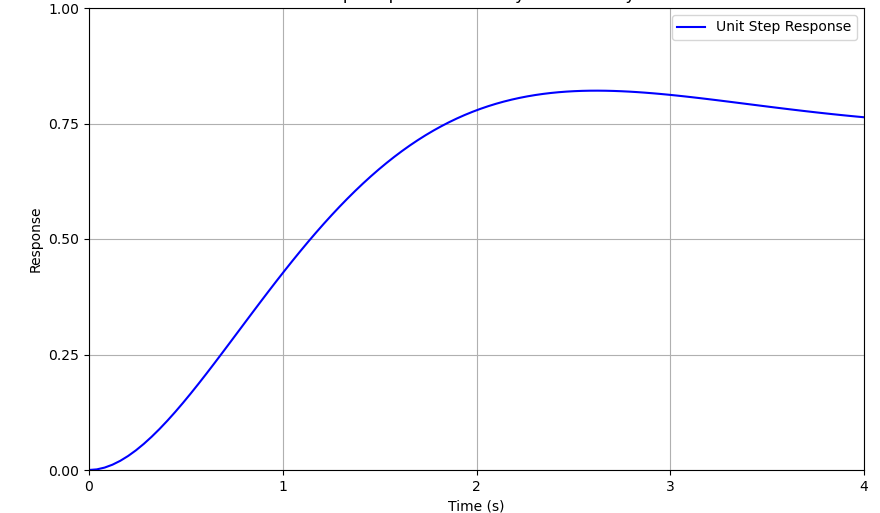
\includegraphics[width=5cm]{figs/fig1.png}
    \caption{}
    \end{figure}
\begin{enumerate}
\item 0.5
\item 2
\item 4
\item 6
\end{enumerate}
\newpage
%28
\item The open loop transfer function of a unity feedback system is given by $G\brak{s}=\brak{e^{-0.1s}}/s$. The gain margin of this system is
\begin{enumerate}
\item 11.95 dB
\item 17.67 dB
\item 21.33 dB
\item 23.9 dB
\end{enumerate}
%29
\item Match the items in List-I with the items in List-II and select the correct answer using the codes given below the lists.

\begin{tabular}{c c}
\textbf{List I} & \textbf{List II} \\
a. improve power factor & 1. shunt reactor \\
b. reduce the current ripples & 2. shunt capacitor \\
c. increase the power flow in line & 3. series capacitor \\
d. reduce the Ferranti effect & 4. series reactor \\
\end{tabular}

\begin{enumerate}
\item $a \rightarrow 2$, $b \rightarrow 3$, $c \rightarrow 4$, $d \rightarrow 1$
\item $a \rightarrow 2$, $b \rightarrow 4$, $c \rightarrow 3$, $d \rightarrow 1$
\item $a \rightarrow 4$, $b \rightarrow 3$, $c \rightarrow 1$, $d \rightarrow 2$
\item $a \rightarrow 4$, $b \rightarrow 1$, $c \rightarrow 3$, $d \rightarrow 2$
\end{enumerate}
%30
\item Match the items in List-I with the items in List-II and select the correct answer using the codes given below the lists.

\begin{tabular}{c c}
\textbf{List I} & \textbf{List II} \\
a. Short Line & 1. Ohm Relay \\
b. Medium Line & 2. Reactance Relay \\
c. Long Line & 3. Mho Relay \\
\end{tabular}

\begin{enumerate}
\item $a \rightarrow 2$, $b \rightarrow 1$, $c \rightarrow 3$
\item $a \rightarrow 3$, $b \rightarrow 2$, $c \rightarrow 1$
\item $a \rightarrow 1$, $b \rightarrow 2$, $c \rightarrow 3$
\item $a \rightarrow 1$, $b \rightarrow 3$, $c \rightarrow 2$
\end{enumerate}
%31
\item Three generators are feeding a load of 100 MW. The details of the generators are

\begin{tabular}{c c c c}
 & \textbf{Rating\brak{MW}} & \textbf{Efficiency (\%)} & \textbf{Regulation (p.u.) on 100 MVA base} \\
Generator-1 & 100 & 20 & 0.02 \\
Generator-2 & 100 & 30 & 0.04 \\
Generator-3 & 100 & 40 & 0.03 \\
\end{tabular}

In the event of increased load power demand, which of the following will happen?
\begin{enumerate}
\item All the generators will share equal power
\item Generator-3 will share more power compared to Generator-1
\item Generator-1 will share more power compared to Generator-2
\item Generator-2 will share more power compared to Generator-3
\end{enumerate}
%32
    \item A 500 MW, 21 kV, 50 Hz, 3-phase, 2-pole synchronous generator having a rated p.f.=0.9, has a moment of inertia of $27.5 \times 10^3$ kg-m$^2$. The inertia constant \brak{H} will be
    \begin{enumerate}
        \item 2.44 s
        \item 2.71 s
        \item 4.88 s
        \item 5.42 s
    \end{enumerate}
%33
    \item $f\brak{x, y}$ is a continuous function defined over $\brak{x, y} \in \sbrak{0,1} \times \sbrak{0,1}$. Given the two constraints, $x > y^2$ and $y > x^2$, the volume under $f\brak{x, y}$ is
    \begin{enumerate}
        \item $\int_{y=0}^{y=1} \int_{x=y^2}^{x=\sqrt{y}} f\brak{x,y} dx dy$
        \item $\int_{y=x^2}^{y=1} \int_{x=y^2}^{x=1} f\brak{x,y} dx dy$
        \item $\int_{y=0}^{y=1} \int_{x=0}^{x=1} f\brak{x,y} dx dy$
        \item $\int_{y=0}^{y=\sqrt{x}} \int_{x=0}^{\sqrt{y}} f\brak{x,y} dx dy$
    \end{enumerate}
%34
    \item Assume for simplicity that $N$ people, all born in April \brak{\text{a month of 30 days}}, are collected in a room. Consider the event of at least two people in the room being born on the same date of the month, even if in different years, e.g., 1980 and 1985. What is the smallest $N$ so that the probability of this event exceeds 0.5?
    \begin{enumerate}
        \item 20
        \item 7
        \item 15
        \item 16
    \end{enumerate}
%35
    \item A cascade of 3 Linear Time Invariant systems is causal and unstable. From this, we conclude that
    \begin{enumerate}
        \item each system in the cascade is individually causal and unstable
        \item at least one system is unstable and at least one system is causal
        \item at least one system is causal and all systems are unstable
        \item the majority are unstable and the majority are causal
    \end{enumerate}
%36
    \item The Fourier Series coefficients, of a periodic signal $x(t)$, expressed as $x\brak{t} = \sum_{k=-\infty}^{\infty} a_k e^{j2\pi k t/T}$, are given by $a_{-2} = 2 - j1$; $a_{-1} = 0.5 + j0.2$; $a_0 = j2$; $a_1 = 0.5 - j0.2$; $a_2 = 2 + j1$; and $a_k = 0$ for $\abs{k} > 2$. Which of the following is true?
    \begin{enumerate}
        \item $x\brak{t}$ has finite energy because only finitely many coefficients are non-zero
        \item $x\brak{t}$ has zero average value because it is periodic
        \item The imaginary part of $x\brak{t}$ is constant
        \item The real part of $x\brak{t}$ is even
    \end{enumerate}

\end{enumerate}
\end{document}
